\documentclass{article}
\usepackage{amsfonts, amsmath, amssymb, amsthm} % Math notations imported
\usepackage{enumitem}
\usepackage{graphicx}
\usepackage{setspace}
\usepackage{indentfirst}
\usepackage[margin=1in]{geometry}
\graphicspath{{./images/}} % Path to images

% \begin{figure}[htb!]
%      \centering
%      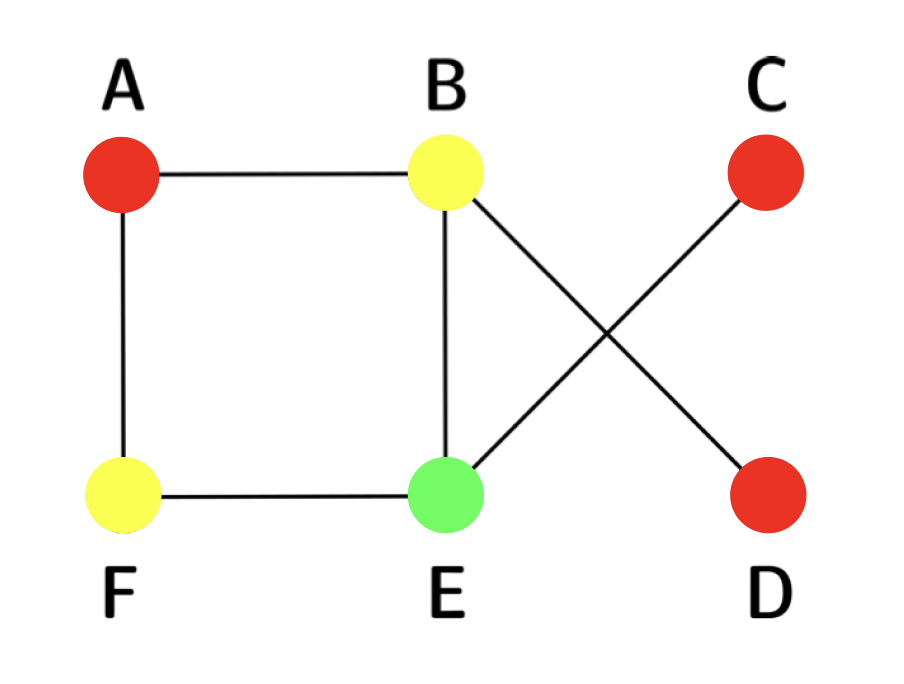
\includegraphics[scale=0.5]{coloring.png}
%      \caption{Coloring of the graph.}
% \end{figure}

\newtheorem{thm}{Theorem}
\newtheorem{proposition}[thm]{Proposition}
\newtheorem{cor}[thm]{Corollary}

% title information
\title{Math 110 HW2}
\author{Neo Lee}
\date{09/09/2023}

\setstretch{1.15}
% main content
\begin{document} 

% placing title information; comment out if using fancyhdr
\maketitle 

\subsection*{Problem 1.}
Suppose $U:=\{(x,x,3x):x\in\mathbb{R}\}$ and $W:=\{(x,-x,-3x):x\in\mathbb{R}\}$. 
\begin{enumerate}[label=(\alph*)]
    \item \begin{proposition}
        $U$ and $W$ are subspaces of $\mathbb{R}^3$.
    \end{proposition}
    \begin{proof}
        
        \textbf{Additive Identity:}
        Let $x = 0$ for both $u\in U$ and $w\in W$. Then $u = (0,0,0)$ and $w = (0,0,0)$, which 
        are both in $U$ and $W$ and are additive identities.

        \textbf{Closed under addition:}
        Let $u_1 = (x_1, x_1, 3x_1), u_2 = (x_2, x_2, 3x_2)\in U$. Then $u_1+u_2 = (x_1+x_2, 
        x_1+x_2, 3x_1+3x_2) = ([x_1+x_2], [x_1+x_2], 3[x_1+x_2])$, which is also in $U$.

        Let $w_1 = (y_1, -y_1, -3y_1), w_2 = (y_2, -y_2, -3y_2)\in W$. Then $w_1+w_2 = (y_1+y_2, 
        -y_1-y_2, -3y_1-3y_2) = ([y_1+y_2], -[y_1+y_2], -3[y_1+y_2])$, which is also in $W$.

        \textbf{Closed under scalar multiplication:}
        Let $u = (x, x, 3x)\in U$ and $c\in\mathbb{R}$. Then $cu = (cx, cx, 3cx) = ([cx], [cx], 
        3[cx])$, which is also in $U$. 

        Let $w = (y, -y, -3y)\in W$ and $c'\in\mathbb{R}$. Then $c'w = (c'y, -c'y, -3c'y) = ([c'y], 
        -[c'y], -3[c'y])$, which is also in $W$.
    \end{proof}
    \item Describe $U+W$ using symbols.
    \begin{proof}[Solution]
        For all $v \in (U+W)$, $v = u + w$ for $u\in U, w\in W$.
    \end{proof}
    \item Describe $U+ W$ without symbols.
    \begin{proof}[Solution]
        For every element in the set $U+W$, it is the sum of an element in $U$ and an element in $W$.
    \end{proof}
\end{enumerate}

\subsection*{Problem 2.}
Suppose $\mathbb{F}=\mathbb{R}$ or $\mathbb{F} = \mathbb{C}$ and let 
$$U = \{(x,y,x+y,-y,-x)\in\mathbb{F}^5:x,y\in\mathbb{F}\}.$$
Find three subspaces $W_1, W_2, W_3$ of $\mathbb{F}^5$, none of which equals \{0\}, such that 
$\mathbb{F}^5=U\oplus W_1\oplus W_2\oplus W_3$.
\begin{proof}[Solution]
    Notice for all $u\in U$, $u = x(1, 0, 1, 0, -1) + y(0, 1, 1, -1, 0)$, which means $U$ is a span 
    of $(1, 0, 1, 0, -1)$ and $(0, 1, 1, -1, 0)$. Now we just need to define $W_1, W_2, W_3$ as 
    the span of any three linearly independent vectors in $\mathbb{F}^5$ that are not in $U$. 
    Let $W_1 = \emph{span}(0, 0, 1, 0, 0), W_2 = \emph{span}(0, 0, 0, 1, 0), W_3 = 
    \emph{span}(0, 0, 0, 0, 1)$. Then $W_1, W_2, W_3$ are subspaces of $\mathbb{F}^5$ and 
    all the five vectors are linearly independent. We can check it by row reducing the matrix 
    with these five vectors as column vectors, but we will omit here since it is trivial.

    Now we have defined our subspaces $U, W_1, W_2, W_3$, we will show that $\mathbb{F}^5 = 
    U\oplus W_1\oplus W_2\oplus W_3$. Let $v \in \mathbb{F}^5$, then we can write $v$ as a linear 
    combination of $u\in U, w_1\in W_1, w_2\in W_2, w_3\in W_3$, which in turns is 
    a linear combination of the five vectors we defined above. Since the five vectors are linearly 
    independent, the linear combination is unique. Therefore, $\mathbb{F}^5 = U\oplus W_1\oplus 
    W_2\oplus W_3$.
\end{proof}

\subsection*{Problem 3.}
\begin{proposition}
    Let $V$ be a vector space over $\mathbb{F}$. Suppose that $1+1\neq 0$ in $\mathbb{F}$ and the 
    list $v_1,v_2,v_3,v_4$ is linearly independent in $V$. Then the list $v_1-v_2,v_1+v_2,v_3-v_2
    ,v_4-v_1$ is also linearly independent in $\mathbb{V}$.
\end{proposition}
\begin{proof}
    We proceed by showing that the zero vector can only be written as a trivial linear 
    combination of $v_1-v_2,v_1+v_2,v_3-v_2,v_4-v_1$. Suppose there exists $a_1, a_2, a_3, a_4\in 
    \mathbb{F}$ such that $a_1(v_1-v_2) + a_2(v_1+v_2) + a_3(v_3-v_2) + a_4(v_4-v_1) = 0$. Then
    \begin{align*}
        a_1(v_1-v_2) + a_2(v_1+v_2) + a_3(v_3-v_2) + a_4(v_4-v_1) &= 0\\
        (a_1+a_2-a_4)v_1 + (-a_1+a_2-a_3)v_2 + a_3v_3 + a_4v_4 &= 0.
    \end{align*}    
    
    Now since $v_1, v_2, v_3, v_4$ are linearly independent, $(a_1+a_2-a_4), (-a_1+a_2-a_3), a_3, 
    a_4$ must all be zero. Now we solve the equations of 
    \begin{align*}
        a_1+a_2-a_4 &= 0\\
        -a_1+a_2-a_3 &= 0\\
        a_3 &= 0\\
        a_4 &= 0.
    \end{align*}
    Solving the linear equations, which we omit here, we get $a_1 = a_2 = a_3 = a_4 = 0$. 
    Therefore, the list $v_1-v_2, v_1+v_2, v_3-v_2, v_4-v_1$ is linearly independent.
\end{proof}

\subsection*{Problem 4.}
Does the statement of Problem 3 still hold if we replace "linearly independent" by "a basis"?
\begin{proof}[Solution]
    We know $dimV = 4$ because the length of the basis $v_1, v_2, v_3, v_4$ is 4. Now, from 
    the previous question, we know that $v_1-v_2, v_1+v_2, v_3-v_2, v_4-v_1$ is linearly 
    independent in $V$. Since the length of the list is also 4, it must be a basis of $V$.
\end{proof}

\subsection*{Problem 5.}
\begin{proposition}
    The space $\mathbb{R}^{[0,1]}$ is infinite-dimensional.
\end{proposition}
\begin{proof}
    Notice that a vector space is finite-dimensional if all its subspaces are finite-dimensional. 
    Now we consider the subspace $\mathcal{P}(x)$, the set of polynomial functions that map from 
    $[0,1]$ to $\mathbb{R}$. Assume for the sake of contradiction that $\mathcal{P}(x)$ is finite 
    and let $dim\mathcal{P} = n$. Then we have $x, x^2, \dots, x^n$, which are all linearly 
    independent and with a total length of $n$, which form the basis of $\mathcal{P}$. Now consider 
    the function $x\mapsto x^{n+1}$, which is still in the subspace $\mathcal{P}$ but not in the 
    span of $x, \dots, x^n$. Hence, by contradiction, $x, \dots, x^n$ does not span the entire 
    subspace $\mathcal{P}$, and $\mathcal{P}$ is infinite dimensional. Therefore, the 
    vector space $\mathbb{R}^{[0,1]}$ is infinite-dimensional as well.
\end{proof}

\end{document}
